\section{Fine Grain Pipelining}
In order to further boost the performance of this floating point multiplier, an additional pipeline register has been inserted in the second stage just after the multiplier. In this case, however, it has been explicitly coded instead of relying on the automatic retiming tool.

\autoref{tab:stage2} shows a full comparison of timing and area requirements as the number of pipeline stages increase. The alternative command \texttt{compile\_ultra -retime} has been compared with \texttt{optimize\_registers} for the first case: the latter has proven to be more effective in minimizing delay. In order to correctly carry out the compilation using \texttt{compile\_ultra} it is necessary to issue \texttt{set\_optimize\_registers} first. The results are shown in table \autoref{tab:stage2_opt_vs_ultra}. 

Synthesis with additional pipeline registers has been performed using \texttt{optimize\_registers}, implicit in the table below.

\begin{table}[htbp]
    \centering
	\begin{tabular}{|r|r|r|r|r|}
	\hline
	                       &\texttt{NPIPE=1} & \texttt{NPIPE=2} & \texttt{NPIPE=4} & \texttt{NPIPE=6}\\\hline
	Delay (ns)                  & 0.78             & 0.71             & 0.68             & 0.72 \\\hline
    Total area  ($\mu$m$^2$)           & 5329             & 5595             & 5793             & 6070 \\\hline
    Combinational area  ($\mu$m$^2$)   & 3068             & 3039             & 2991             & 2978 \\\hline
	\end{tabular}
	\caption{Critical path delay and area with the hardcoded register in the second stage and a varying \texttt{NPIPE} using \texttt{optimize\_registers}}
	\label{tab:stage2}
\end{table}

\begin{table}[htbp]
	\centering
	\begin{tabular}{|r|r|r|}
		\hline
		& compile\_ultra 	& optimize\_registers \\\hline
		Delay(ns)     		& 1.37				& 0.78  \\\hline
		Total area  ($\mu$m$^2$)        	& 4395 				& 5329   \\\hline
		Combinational area  ($\mu$m$^2$)	& 3065 				& 3068   \\\hline
	\end{tabular}
	\caption{Critical path delay and area with the hardcoded register in the second stage with \texttt{NPIPE} equal to 1 comparing \texttt{compile\_ultra} and \texttt{optimize\_registers}}
	\label{tab:stage2_opt_vs_ultra}
\end{table}


It is possible to see how the delay decreases as more registers are added. This is no longer true for \texttt{NPIPE} = 6, since the overhead introduced by the setup, skew and jitter times of the new registers overweighs the advantages provided by theoretical pipelining.\\
It is interesting to notice how while the total area increases, the combinational area, instead, steadily decreases. This is possibly due to the fact that the pipelining technique relaxes not only the timing constraints of the combinational logic, but also the power constraints: since the combinational paths are broken into smaller sections, there is less necessity for buffers and also the cells themselves no longer need as much driving strength, thus can also be smaller.


\paragraph{Critical path delay distribution}
\autoref{fig:hist2} and \autoref{fig:hist6} show how worst path delays tend to accumulate towards the shortest one as the degree of pipelining increases. This is a general pattern seen when applying this technique.
\begin{figure}[htbp]
    \begin{subfigure}{0.5\textwidth}
	   \centering
	   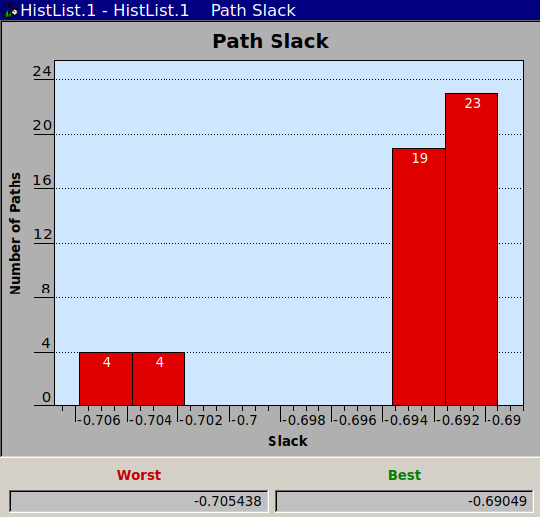
\includegraphics[width=\textwidth]{chapter1/images/npipe2.png}
	   \caption{Worst path distribution with \texttt{NPIPE=2}}
	   \label{fig:hist2}
    \end{subfigure}
    \begin{subfigure}{0.5\textwidth}
        \centering
	    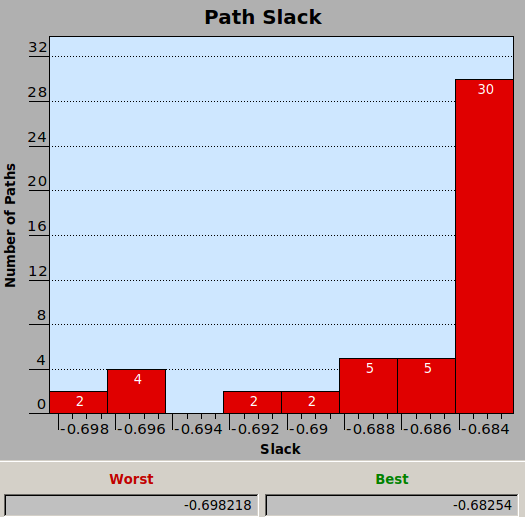
\includegraphics[width=\textwidth]{chapter1/images/npipe6.png}
	    \caption{Worst path distribution with \texttt{NPIPE=6}}
	    \label{fig:hist6}
	\end{subfigure}
\end{figure}
